\chapter{Gestion des événement   }
\addcontentsline{toc}{chapter}{Chapitre 4 : Gestion des événement  }

\section*{Introduction}
\addcontentsline{toc}{section}{Introduction}
Dans ce chapitre, nous allons étudier en profondeur le troisième sprint de notre projet. Toutefois, avant de gérer les événements, il est nécessaire de gérer les catégories, afin de pouvoir classer chaque événement selon sa catégorie.
\section{Organisation du sprint}
Notre chapitre est composée par :\\
\textbf{Sprint 3 :} Gestion des événement (CRUD).
\section{Sprint 3 : Gestion des événement (CRUD)}
\subsection{Objectif du sprint}\\
xL'objectif de ce sprint est de Création, modification, suppression et affichage des événements .et aussi de creation et de modification , suppression des catégories.

\subsection{Sprint backlog}
Le 3éme sprint s’étend du 22 février au 04 mars. Le tableau suivant représente le backlog de ce sprint:
\begin{table}[h!]
\renewcommand{\arraystretch}{1.6}
\setlength{\tabcolsep}{5pt}
\centering
\begin{tabular}{|c|c|m{7cm}|c|c|}
\hline
\textbf{ID} & \textbf{Sprint} & \textbf{User Story} & \textbf{Priorité} & \textbf{Complexité} \\
\hline

\multirow{11}{*}{3} & \multirow{11}{*}{\parbox{3cm}{\centering Gestion des événements}}
& En tant qu’administrateur, je veux créer des catégories. & Élevée & Faible \\
\cline{3-5}
&& En tant qu’administrateur, je veux modifier des catégories. & Moyenne & Faible \\
\cline{3-5}
&& En tant qu’administrateur, je veux supprimer des catégorie. & Moyenne & Faible\\
\cline{3-5}
&& En tant qu’administrateur, je veux consulter les catégories. & Moyenne & Trés  faible \\
\cline{3-5}
&& En tant qu’administrateur, je veux modifier des événements. & Élevée & Moyenne \\
\cline{3-5}
& & En tant qu’administrateur, je veux supprimer des événements. & Élevée & Moyenne \\
\cline{3-5}
& & En tant qu’administrateur, je veux consulter des événements. & Moyenne  & Trés faible \\
\cline{3-5}
& & En tant qu’administrateur, je veux approuver des événements. & Élevée & Faible \\
\cline{3-5}
& & En tant que gestionnaire, je veux créer mon événements. & Élevée & Moyenne \\
\cline{3-5}
& & En tant que gestionnaire, je veux modifier mon événements. & Moyenne & Moyenne \\
\cline{3-5}
& & En tant que gestionnaire, je veux supprimer mon  événements. & Moyenne & Faible \\
\hline

\end{tabular}
\end{table}
\subsection{Implémentation du sprint 3}
\subsubsection{Spécification des besoins}
Dans cette section, nous identifions les besoins de notre  sprint, à travers :
\begin{itemize}
    \item les diagrammes de cas d’utilisation,
    \item les descriptions textuelles associées,
    \item les diagrammes de séquences système.
\end{itemize}

\textbf {La figure ci-dessous représente le diagramme de cas d’utilisation de ce sprint par rapport de l'administrateur.}
\begin{figure}[H]
    \centering
    \includegraphics[width=0.6\linewidth]{projet/images/Sprint 3/gérer les catégorie.png}
    \caption{Diagramme des cas d’utilisation gestion des catégorie "Administrateur" }
    \label{fig:Adminee }
\end{figure}

Ce diagramme décrit le processus de gestion d'évenement pour l'administrateur. Nous détaillons ci-après ce cas d’utilisation sous forme textuelle :
\begin{longtable}{|>{\bfseries}p{4cm}|p{10cm}|}
\hline
Cas d’utilisation &  Créer un catégorie \\
\hline
Acteurs & Administrateur \\
\hline
Précondition & Authentification préalable\\
\hline
Post-condition & categorie ajouter dans le systéme\\
\hline
Scénario principal & 
\begin{enumerate}
  \item   L’administrateur clique sur le bouton "Gérer les catégorie"
    \item le systeme affiche le formulaire de création
  \item   L’administrateur saisit les informations nécessaires et valide et clique sur button "Ajouter"
  \item Le système enregistre la nouvelle catégorie.

\end{enumerate} 
\hline
Scénario alternatif & 
\begin{enumerate}
    \item Le formulaire est soumis avec des champs invalides
    \item Le système affiche un message d’erreur.
\end{enumerate}
 \hline
\caption{Description textuelle du cas d’utilisation pour créer un catégorie }
\end{longtable}
\clearpage
\begin{longtable}{|>{\bfseries}p{4cm}|p{10cm}|}
\hline
Cas d’utilisation &  Modifier un catégorie \\
\hline
Acteurs & Administrateur \\
\hline
Précondition & Authentification préalable\\
\hline
Post-condition & categorie est en mise a jour dans le systéme\\
\hline
Scénario principal & 
\begin{enumerate}
  \item  L’administrateur sélectionne une catégorie à modifier
    \item Le système affiche les informations de la catégorie
  \item   L’administrateur modifie les champs désirés et valide.
  \item  Le système met à jour les données

\end{enumerate} 
\hline
Scénario alternatif & 
\begin{enumerate}
    \item Champs invalides.
    \item Le système affiche un message d’erreur.
\end{enumerate}
 \hline
\caption{Description textuelle du cas d’utilisation pour   Modifier un catégorie }
\end{longtable}


\begin{longtable}{|>{\bfseries}p{4cm}|p{10cm}|}
\hline
Cas d’utilisation &  Supprimer un catégorie \\
\hline
Acteurs & Administrateur \\
\hline
Précondition & Authentification préalable\\
\hline
Post-condition & categorie est supprrimer dans le systéme\\
\hline
Scénario principal & 
\begin{enumerate}
  \item  L’administrateur sélectionne une catégorie à supprimer
    \item Le système demande confirmation 
  \item   L’administrateur confirme la suppréssion.
  \item  Le système supprime la catégorie

\end{enumerate} 
\hline
Scénario alternatif & 
\begin{enumerate}
    \item l'administrateur annule la suppression 
    \item Le système affiche un message d’erreur.
\end{enumerate}
 \hline
\caption{Description textuelle du cas d’utilisation pour  Supprimer un catégorie }
\end{longtable}



\begin{longtable}{|>{\bfseries}p{4cm}|p{10cm}|}
\hline
Cas d’utilisation &  Consulter un catégorie \\
\hline
Acteurs & Administrateur \\
\hline
Précondition & Authentification préalable\\
\hline
Post-condition & les catégories sont affichées
\hline
Scénario principal & 
\begin{enumerate}
  \item L’administrateur accède à la page des catégories.
    \item Le système affiche la liste des catégories existantes.  
\end{enumerate} 
\hline
Scénario alternatif & Néant

 \hline
\caption{Description textuelle du cas d’utilisation pour   Consulter un catégorie }
\end{longtable}
\begin{figure}[H]
    \centering
    \includegraphics[width=0.6\linewidth]{projet/images/Sprint 3/gérer les evenement.png}
    \caption{Diagramme des cas d’utilisation gestion d'évenement "Administrateur" }
    \label{fig:Adminee }
\end{figure}
Ce diagramme décrit le processus de gestion d'évenement pour l'administrateur. Nous détaillons ci-après ce cas d’utilisation sous forme textuelle :

\begin{longtable}{|>{\bfseries}p{4cm}|p{10cm}|}
\hline
Cas d’utilisation &  Modifier un évenement \\
\hline
Acteurs & Administrateur \\
\hline
Précondition & Authentification préalable\\
\hline
Post-condition & évenement Modifier\\
\hline
Scénario principal & 
\begin{enumerate}
  \item  L’administrateur choisit l'évenement à modifier et clique sur son bouton de modification.

  \item Le système affiche le formulaire de modification d’un évenement

  \item L’administrateur modifie les informations du l'évenement et le soumet
  \item Le système vérifie les information setmet à jour les données d'évenement 
  \item Le système affiche un message de succès
\end{enumerate} 
\hline
Scénario alternatif & L’administrateur soumet le formulaire avec des informations incomplètes ou incorrectes \\
 \hline 
\caption{Description textuelle du cas d’utilisation pour  Modifier un évenement  }
\end{longtable}



\begin{longtable}{|>{\bfseries}p{4cm}|p{10cm}|}
\hline
Cas d’utilisation &  Supprimer un évenement \\
\hline
Acteurs & Administrateur \\
\hline
Précondition & Authentification préalable\\
\hline
Post-condition & évenement Supprimer\\
\hline
Scénario principal & 
\begin{enumerate}
  \item  L’administrateur choisit l'évenement à supprimer et clique sur son bouton de suppression.

  \item Le système demande une confirmation de la suppression

  \item  L’administrateur confirme la suppression
  \item Le système supprime l'évenement 
  \item Le système affiche un message de succès
\end{enumerate} 
\hline

Scénario alternatif & L’administrateur annule la confirmation
 \hline
\caption{Description textuelle du cas d’utilisation pour  Supprimer l'évenement }
\end{longtable}


\begin{longtable}{|>{\bfseries}p{4cm}|p{10cm}|}
\hline
Cas d’utilisation &  Consulter un évenement \\
\hline
Acteurs & Administrateur \\
\hline
Précondition & Authentification préalable\\
\hline
Post-condition & La liste des évenement  est affichée\\
\hline
Scénario principal & 
\begin{enumerate}
  \item  L’administrateur accède a partie de gestion d'évenement 

  \item Le système affiche un tableau qui contient tous les évenements

\end{enumerate} 
\hline
Scénario alternatif & Néant
 \hline
\caption{Description textuelle du cas d’utilisation pour  Consulter l'évenement }
\end{longtable}


\begin{longtable}{|>{\bfseries}p{4cm}|p{10cm}|}
\hline
Cas d’utilisation & Approuver un événement \\
\hline
Acteur & Administrateur \\
\hline
Précondition & L’administrateur est authentifié dans le système. \\
\hline
Post-condition & L’événement est marqué comme "Approuvé" et devient visible au public. \\
\hline
Scénario principal & 
\begin{enumerate}
  \item L’administrateur accède à la liste des événements.
  \item Le système affiche la liste des événements.
  \item L’administrateur sélectionne un événement en attente
 
  \item L’administrateur clique sur le bouton "accepter" ou "réfuser".
  \item Le système met à jour le statut de l’événement en "Approuvé".
  \item Le système affiche un message de confirmation de l’approbation.
\end{enumerate} 
\hline
Scénario alternatif & 
\begin{itemize}
  \item Si l’événement est déjà approuvé, le système affiche un message indiquant que l’événement a déjà été approuvé et empêche toute modification du statut.
\end{itemize} 
\hline
\caption{Description textuelle du cas d’utilisation pour Approuver un événement}
\end{longtable}
\textbf {La figure ci-dessous représente le diagramme de cas d’utilisation de ce sprint par rapport de l'administrateur.}
\begin{figure}[H]
    \centering
    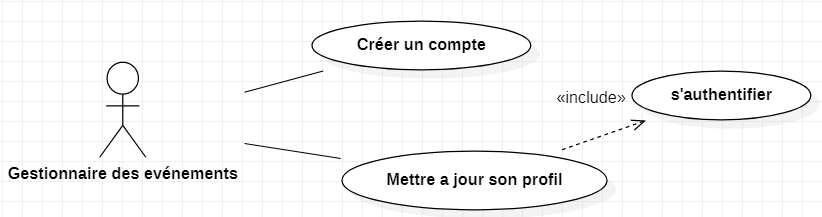
\includegraphics[width=0.6\linewidth]{projet/images/Sprint 3/gestionnaire.png}
    \caption{Diagramme des cas d’utilisation gestion d'évenement "Gestionnaire" }
    \label{fig:Adminee }
\end{figure}
Ce diagramme décrit le processus de gestion d'évenement pour le Gestionnaire. Nous détaillons ci-après ce cas d’utilisation sous forme textuelle :

\begin{longtable}{|>{\bfseries}p{4cm}|p{10cm}|}
\hline
Cas d’utilisation & créer un événement \\
\hline
Acteur & Gestionnaire d'évenement \\
\hline
Précondition & Le gestionnaire est authentifié \\
\hline
Post-condition & L’événement est ajouté à la base de données \\
\hline
Scénario principal & 
\begin{enumerate}
  \item Le gestionnaire clique sur "Ajouter un événement".
  \item Le système affiche le formulaire de création.
  \item  Le gestionnaire remplit les champs requis et valide et clique sur button "Enregistrer l'évenement"
  \item Le système enregistre l’événement.
  \item  Un message de confirmation s’affiche.

\end{enumerate} 
\hline
Scénario alternatif & 
\begin{itemize}
  \item Champs invalides ou manquants.
  \item Le système affiche un message d’erreur
\end{itemize} 
\hline
\caption{Description textuelle du cas d’utilisation pour créer un événement}
\end{longtable}


\begin{longtable}{|>{\bfseries}p{4cm}|p{10cm}|}
\hline
Cas d’utilisation & Modifier un événement \\
\hline
Acteur & Gestionnaire d'évenement \\
\hline
Précondition & Le gestionnaire est authentifié \\
\hline
Post-condition & L’événement est mis à jour \\
\hline
Scénario principal & 
\begin{enumerate}
  \item Le gestionnaire sélectionne un événement à modifier.
  \item Le système affiche les détails de l’événement
  \item  Le gestionnaire modifie les champs désirés et valide
  \item Le système met à jour l’événement.
  \item Un message de confirmation s’affiche.
\end{enumerate} 
\hline
Scénario alternatif & 
\begin{itemize}
  \item Champs invalides .
  \item Le système affiche un message d’erreur
\end{itemize} 
\hline
\caption{Description textuelle du cas d’utilisation pour  Modifier un événement}
\end{longtable}


\begin{longtable}{|>{\bfseries}p{4cm}|p{10cm}|}
\hline
Cas d’utilisation & Supprimer un événement \\
\hline
Acteur & Gestionnaire d'évenement \\
\hline
Précondition & Le gestionnaire est authentifié \\
\hline
Post-condition & L’événement est supprimer \\
\hline
Scénario principal & 
\begin{enumerate}
  \item Le gestionnaire sélectionne un événement à supprimer.
  \item  Le système demande confirmation.
  \item Le gestionnaire confirme.
  \item Le système supprime l’événement.
  \item Un message de confirmation s’affiche.
\end{enumerate} 
\hline
Scénario alternatif & 
\begin{itemize}
  \item le gestionnaire annule  .
  \item Le système annule l'operation
\end{itemize} 
\hline
\caption{Description textuelle du cas d’utilisation pour  supprimer un événement}
\end{longtable}


\begin{longtable}{|>{\bfseries}p{4cm}|p{10cm}|}
\hline
Cas d’utilisation & Consulter un événement \\
\hline
Acteur & Gestionnaire d'évenement \\
\hline
Précondition & Le gestionnaire est authentifié \\
\hline
Post-condition & Les événements sont affichés \\
\hline
Scénario principal & 
\begin{enumerate}
  \item Le gestionnaire accède à la page gérer les événements.
  \item  Le système affiche la liste des évenements
 
\end{enumerate} 
\hline

\caption{Description textuelle du cas d’utilisation pour  consulter les  événement}
\end{longtable}
\textbf{Les figures ci-après illustrent les diagrammes de séquences systèmes des différents cas d’utilisation de notre 3éme sprint.}
\begin{figure}[H]
    \centering
    \includegraphics[width=1\linewidth]{projet/Crée un categorie.png}
    \caption{Diagramme de séquence système Crée un catégorie}
    \label{fig:diagramme3}
\end{figure}
\begin{figure}[H]
    \centering
    \includegraphics[width=1\linewidth]{projet/Modifier un categorie.png}
    \caption{Diagramme de séquence système Modifier un catégorie}
    \label{fig:diagramme3}
\end{figure}
\begin{figure}[H]
    \centering
    \includegraphics[width=1\linewidth]{projet/Supprimer un categorie.png}
    \caption{Diagramme de séquence système Supprimer un catégorie}
    \label{fig:diagramme3}
\end{figure}
\begin{figure}[H]
    \centering
    \includegraphics[width=1\linewidth]{projet/Consulter un categorie.png}
    \caption{Diagramme de séquence système Consulter un catégorie}
    \label{fig:diagramme3}
\end{figure}
\begin{figure}[H]
    \centering
    \includegraphics[width=1\linewidth]{projet/Supprimer un évenement.png}
    \caption{Diagramme de séquence système Modifier des évenement}
    \label{fig:diagramme3}
\end{figure}
\begin{figure}[H]
    \centering
    \includegraphics[width=1\linewidth]{projet/Supprimer un évenement.png}
    \caption{Diagramme de séquence système Supprimer des évenement}
    \label{fig:diagramme3}
\end{figure}
\begin{figure}[H]
    \centering
    \includegraphics[width=1\linewidth]{projet/Consulter un évenement.png}
    \caption{Diagramme de séquence système Consulter un évenement}
    \label{fig:diagramme3}
\end{figure}
\begin{figure}[H]
    \centering
    \includegraphics[width=1\linewidth]{projet/images/Sprint 3/Admin Approver evenement diagram sequance.png un évenement.png}
    \caption{Diagramme de séquence système Approver un évenement}
    \label{fig:diagramme3}
\end{figure}
